\section{Related work}
\label{seq:relatedwork}

Computing neighborhoods in a point cloud is a non-trivial task due to the irregular nature of the data itself.
The neighborhood of a given data point is composed of all the surrounding points meeting a certain condition, and it provides information about the local structure of the point cloud, which is essential in its processing____.
The most common neighboring methods encountered in the state-of-the-art literature are two:
the fixed-radius neighborhood____ and the \gls{KNN}____.
While the former queries the point cloud to retrieve all the points inside a previously defined kernel, the latter computes the $k$-nearest points using any valid metric.

Regarding the fixed-radius neighborhoods, the typical approach is to use a spherical neighborhood, composed of all the points whose Euclidean distance to the queried point is less than $R$.
Note that different distances than the $L_2$ norm can be used, such as the $L_1$ norm or the $L_{\infty}$ norm, for generating cubic neighborhoods, for example.
Another variation is to ignore the third spatial dimension (typically the vertical, $z$), producing a cylindrical neighborhood, often used in point clouds obtained from airborne platforms____.
While these two kernels are the most common, any custom geometry can be defined and used to carry out the queries: cubes, and their 2D counterpart squares, toroids, and so on.

Concerning the $k$-nearest neighbors, the method needs the parameter $k$, which is the number of neighbors to be found, and the neighborhood is composed of the $k$-closest points to the queried point.
If the point being queried is located in a low-density area, the $k$-closest neighbors may include points too far away to be geometrically meaningful.
This could be detrimental to the quality of the local descriptors computed on the point, such as linearity, planarity, or eigenentropy.
To overcome this issue, some authors use a mixed approach. For example,____ employs a fixed-radius sphere as a kernel, but only $k$ randomly selected neighbors are included.

Which type of neighborhood to use depends on the application.
When processing point clouds, the neighborhood computation is usually the most computationally expensive operation____, so choosing the correct approach is crucial in terms of accuracy and saving computing time.
Both types of search methods depend on a parameter, which must be chosen carefully.
Due to the irregular nature of point clouds, a fixed-radius search can be appropriate for some areas of the cloud but may fail in others.
This occurs because of the variations of point densities across a single dataset.
To avoid this problem, some authors suggest the use of different scales across the dataset to retrieve the neighborhood.
For example,____ presented a way to adapt the query parameter for each point.
An improvement of this technique is proposed in____ for \KNN queries and in____ for fixed-radius neighborhoods.
Nevertheless, the computational cost is still significant.

To reduce query times, some authors rely on stochastic sampling methods, such as the Poisson Disk Sampling____, which produces evenly distributed sets of points in a specific region. This is the case of____, where the random sampling is also accelerated using GPU support to keep a high number of neighbors while reducing the computation times.
To compute multiscale neighborhoods in reasonable times,____ opted to perform a subsampling of the dataset by using a grid, which allows them to control the size of the neighborhoods.
In the realm of real-time applications,____ used a GPU-accelerated algorithm to detect obstacles for mobile vehicles.
The hardware accelerated methods are also useful to process massive point clouds, as is the case of____, where GPUs are used to accelerate the computation of triangular irregular networks.

Notably, the method used in____ exploits the geometry of the scanlines to retrieve the spherical neighborhood in $\bigO{1}$.
By knowing the characteristics of the sensor, the point cloud is transformed into a convenient space where each point has two indexes: one for the scanline it belongs to and another for its position inside the scanline.
Nevertheless, this method is only valid when the sensor is known and its scanning pattern is regular and predictable.

The naïve method for computing the neighborhoods is checking for every point in the dataset whether it meets the conditions to be part of the neighborhood or not.
This method could be suitable if the point clouds are composed of a few hundred points (see \cref{fig:brute-force-vs-indexing}), but modern point clouds have millions of points, making this approach unfeasible.

\begin{figure}
  \centering
  % This file was created with tikzplotlib v0.10.1.
  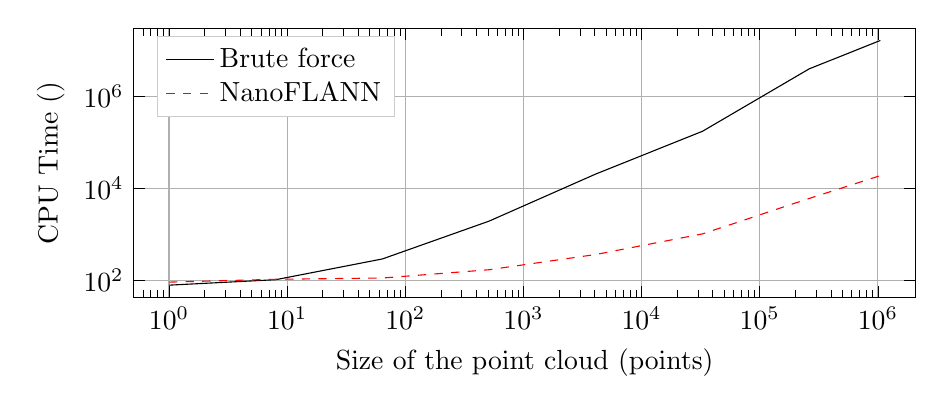
\begin{tikzpicture}

    \definecolor{darkgray176}{RGB}{176,176,176}
    \definecolor{lightgray204}{RGB}{204,204,204}

    \begin{axis}[
        width=0.95\linewidth,
        height=5cm,
        legend cell align={left},
        legend style={
          fill opacity=1.0,
          draw opacity=1,
          text opacity=1,
          at={(0.03,0.97)},
          anchor=north west,
          draw=lightgray204
        },
        xmajorgrids,
        ymajorgrids,
        log basis x={10},
        log basis y={10},
        tick pos=both,
        x grid style={darkgray176},
        xlabel={Size of the point cloud (points)},
        xmin=0.5, xmax=2097152,
        xmode=log,
        xtick style={color=black},
        y grid style={darkgray176},
        ylabel={CPU Time (\si{\nano\second})},
        ymin=43.2831024242217, ymax=29885537.5292166,
        ymode=log,
        % grid=both,
        ytick style={color=black}
      ]
      \addplot [black]
      table {%
        1 79.7506
        8 104.771
        64 295.298
        512 1954.6
        4096 20566.1
        32768 173845
        262144 3929480
        1048576 16219800
      };
      \addlegendentry{Brute force}
      \addplot [red, dashed]
      table {%
        1 92.844
        8 106.926
        64 113.922
        512 172.339
        4096 368.943
        32768 1032.76
        262144 6066.56
        1048576 18953.4
      };
      \addlegendentry{NanoFLANN}
    \end{axis}

  \end{tikzpicture}
  \caption{Spherical query (\qty{2.5}{\meter} radius) in a synthetic point cloud of dimensions \qtyproduct{100 x 100 x 50}{\meter} on a system with a 6-core (12-threads) Intel Core i7-9750H and \qty{32}{\giga\byte} DDR4 memory at \qty{2666}{\mega\hertz}.}
  \label{fig:brute-force-vs-indexing}
\end{figure}

To overcome this issue, several data structures were created to speed up the query times.
The \KDTree____ is a tree-based data structure in which each node has a maximum of two children.
In the \KDTree, the data domain is partitioned by using ($k$-1)-dimensional planes, and each division created by each plane corresponds to a node of the tree.
The \Octree____ is also a tree-based data structure, but each node has 8 children.
The space partitioning in this case is carried out using voxels: The root of the \Octree is a voxel whose size's length is the larger edge of the minimum bounding box of the dataset.
Each voxel is then subdivided into 8 equal voxels by halving its length.
The partitioning is usually stopped when a fixed number of data for a given voxel is reached.
Other not-so-common data structures are the Ball Tree____ and the \Rtree____.
The Ball Tree can be thought of as the same as a \KDTree, but using ($k$-1)-dimensional spheres instead of planes.
The \Rtree is similar to the \Octree, but the space partitioning is carried out by computing smaller bounding boxes for each level of the tree.
To check whether two elements are nearby, the collision of the bounding boxes must be computed, which usually is a computationally cheap operation.

The most commonly used of the aforementioned data structures to carry out neighboring searches are the \KDTree and the \Octree.

\KDTree is known for its effectiveness in multidimensional data for nearest-neighbor searches____, having an average complexity of $\bigO{\log{N}}$ for finding the nearest neighbor in a point cloud with $N$ points.
Nevertheless, this complexity can be limiting____.

\Octree is widely utilized for organizing point clouds into voxels, simplifying the exploitation of its structure for neighbor searching____.
It is also used in indexing structures for massive point clouds, enhancing the efficiency of spatial indexing____, and neighbor searching methods for 3D point clouds, particularly in the context of \gls{LiDAR} data____.

Furthermore, in the context of graph-based networks and point cloud analysis, \KDTree is utilized for conducting point-to-node $k$-nearest-neighbor searches.
This allows for the systematic adjustment of the network's receptive field____.
Additionally, \KDTree is used in the establishment of a three-dimensional point cloud registration based on entropy and particle swarm optimization, where the relationship of points is established by \KDTree for finding the $k$-nearest neighbor of a point____.
\Octree, on the other hand, has been used in the context of 3D change detection, where it is employed for adaptive thresholds based on local point cloud density____.

Both \KDTree and \Octree play crucial roles in neighbor searches in point clouds, however, to the best of our knowledge, they have been reviewed only twice in the literature.
In the work by Elseberg et al.____, the performance of five implementations of \KDTree, one \Octree, and one \Rtree is compared when used for k-nearest neighbors and fixed-radius queries, in the context of shape registration in synthetic and real point cloud data.
The other review is presented by Lawson et al.____, where a single unstructured mesh composed of \num{152.7} million nodes and \num{152.1} million hexahedral elements is used as a study case.
In that review, a deep comparison between 20 open-source C/\Cpp libraries implementing different search methods is presented.
However, the study uses synthetic data with an unknown spatial distribution.

While the aforementioned studies presented are exhaustive, some questions remain unanswered:
How do the different data structures perform in real-world point clouds?
How do they perform in different types of point clouds?
How do the density and distribution of points affect the performance of neighboring search methods?
Is the performance different in \KNN and fixed-radius queries?
Can a novel data structure outperform current state-of-the-art data structures?

In this work, we aim to answer these questions by comparing different methods for performing neighborhood search, while proposing a new data structure to perform neighbor searches in three-dimensional point clouds.